	%%%%%%%%%%%%%%%%%%%%%%%%%%%%%%%%%%%%%%%%%
% HW Template
% LaTeX Template
% Version 1.0 (19/10/18)
% Modified by
% Erdem TUNA
% Halil TEMURTAŞ 
% Enes TAŞTAN 
%%%%%%%%%%%%%%%%%%%%%%%%%%%%%%%%%%%%%%%%%
%
%----------------------------------------------------------------------------------------
%	PACKAGES AND OTHER DOCUMENT CONFIGURATIONS
%----------------------------------------------------------------------------------------
\documentclass[a4paper,12pt]{article}
%-----packages------
\usepackage[a4paper, total={6.5in, 8.5in}]{geometry}
\usepackage[english]{babel}
\usepackage[utf8x]{inputenc}
\usepackage{amsmath}
\usepackage{graphicx}
\usepackage[colorinlistoftodos]{todonotes}
\usepackage{gensymb} % this could be problem
\usepackage{float}
\usepackage{fancyref}
\usepackage{subcaption}
\usepackage[toc,page]{appendix} %appendix package
\usepackage{xcolor}
\usepackage{listings}
\usepackage{xspace}
\usepackage{amssymb}
\usepackage{nicefrac}
\usepackage{gensymb}
\usepackage{fancyhdr}
\usepackage{blindtext}  % for dummy text, use \blindtext or \BlindText
\usepackage[final]{pdfpages}  % pdf include
\usepackage{array} %allows more options in tables
\usepackage{pgfplots,pgf,tikz} %coding plots in latex
\usepackage{capt-of} % allows caption outside the figure environment
\usepackage[export]{adjustbox} %more options for adjusting the images
\usepackage{multicol,multirow,slashbox} % allows tables like table1
%\usepackage[hyperfootnotes=false]{hyperref} % clickable references
\usepackage{epstopdf} % useful when matlab is involved
%\usepackage{placeins} % prevents the text after figure to go above figure with \FloatBarrier 
%\usepackage{listingsutf8,mcode} %import .m or any other code file mcode is for matlab highlighting

%-----end of packages

%-----specifications-----
\definecolor{mGreen}{rgb}{0,0.6,0} % for python
\definecolor{mGray}{rgb}{0.5,0.5,0.5}
\definecolor{mPurple}{rgb}{0.58,0,0.82}
\definecolor{mygreen}{RGB}{28,172,0} % color values Red, Green, Blue for matlab
\definecolor{mylilas}{RGB}{170,55,241}

\setcounter{secnumdepth}{5} % how many sectioning levels to assign numbers to
\setcounter{tocdepth}{5}    % how many sectioning levels to show in ToC

\lstdefinestyle{CStyle}{
	commentstyle=\color{mGreen},
	keywordstyle=\color{magenta},
	numberstyle=\tiny\color{mGray},
	stringstyle=\color{mPurple},
	basicstyle=\footnotesize,
	breakatwhitespace=false,         
	breaklines=true,
	frame=single,
	rulecolor=\color{black!40},                 
	captionpos=b,                    
	keepspaces=true,                 
	numbers=left,                    
	numbersep=5pt,                  
	showspaces=false,                
	showstringspaces=false,
	showtabs=false,                  
	tabsize=2,
	language=C
}

\lstset{language=Matlab,%
	%basicstyle=\color{red},
	breaklines=true,%
	frame=single,
	rulecolor=\color{black!40},
	morekeywords={matlab2tikz},
	keywordstyle=\color{blue},%
	morekeywords=[2]{1}, keywordstyle=[2]{\color{black}},
	identifierstyle=\color{black},%
	stringstyle=\color{mylilas},
	commentstyle=\color{mygreen},%
	showstringspaces=false,%without this there will be a symbol in the places where there is a space
	numbers=left,%
	numberstyle={\tiny \color{black}},% size of the numbers
	numbersep=9pt, % this defines how far the numbers are from the text
	emph=[1]{for,end,break},emphstyle=[1]\color{red}, %some words to emphasise
	%emph=[2]{word1,word2}, emphstyle=[2]{style},    
}


\tikzset{
	desicion/.style={
		diamond,
		draw,
		text width=4em,
		text badly centered,
		inner sep=0pt
	},
	block/.style={
		rectangle,
		draw,
		text width=10em,
		text centered,
		rounded corners
	},
	cloud/.style={
		draw,
		ellipse,
		minimum height=2em
	},
	descr/.style={
		fill=white,
		inner sep=2.5pt
	},
	connector/.style={
		-latex,
		font=\scriptsize
	},
	rectangle connector/.style={
		connector,
		to path={(\tikztostart) -- ++(#1,0pt) \tikztonodes |- (\tikztotarget) },
		pos=0.5
	},
	rectangle connector/.default=-2cm,
	straight connector/.style={
		connector,
		to path=--(\tikztotarget) \tikztonodes
	}
}

\tikzset{
	desicion/.style={
		diamond,
		draw,
		text width=4em,
		text badly centered,
		inner sep=0pt
	},
	block/.style={
		rectangle,
		draw,
		text width=10em,
		text centered,
		rounded corners
	},
	cloud/.style={
		draw,
		ellipse,
		minimum height=2em
	},
	descr/.style={
		fill=white,
		inner sep=2.5pt
	},
	connector/.style={
		-latex,
		font=\scriptsize
	},
	rectangle connector/.style={
		connector,
		to path={(\tikztostart) -- ++(#1,0pt) \tikztonodes |- (\tikztotarget) },
		pos=0.5
	},
	rectangle connector/.default=-2cm,
	straight connector/.style={
		connector,
		to path=--(\tikztotarget) \tikztonodes
	}
}
%-----end of specifications-----


%----commands----
\newcommand\nd{\textsuperscript{nd}\xspace}
\newcommand\rd{\textsuperscript{rd}\xspace}
\newcommand\nth{\textsuperscript{th}\xspace} %\th is taken already
\newcommand{\specialcell}[2][c]{ \begin{tabular}[#1]{@{}c@{}}#2\end{tabular}} % for too long table lines

\newcommand{\blankpage}{
	\- \\[9cm]	
	{ \centering \textit{This page intentionally left blank.} \par }
	\- \\[9cm]
}% For Blank Page

\makeatletter
\renewcommand\paragraph{\@startsection{paragraph}{4}{\z@}%
	{-2.5ex\@plus -1ex \@minus -.25ex}%
	{1.25ex \@plus .25ex}%
	{\normalfont\normalsize\bfseries}}
\makeatother
%-----end of commands-----


\pagestyle{fancy}
\fancyhead[LO,LE]{Halil TEMURTAŞ / 2094522 \\ İclal SATICI / 2094407 }
\fancyhead[RO,RE]{\today}
\fancyfoot[RO,RE]{
\includegraphics[width=2.4cm]{images/eelogo}}

\begin{document}
\begin{center}
	\textbf{\large EE407 Process Control \\[0.2cm] HW 3} \\
\end{center}


\begin{enumerate}

	\item
		
			\begin{enumerate}
				\item $ m=2 $, $n=2$ , $m+n+1=5$  
					$$ e^{-\theta s}=1-\theta s+\theta^2 \frac{s^2}{2!}-\theta^3\frac{s^3}{3!}+\theta^4\frac{s^4}{4!} \approx  \frac{a_0+a_1s+a_2s^2}{1+b_1s+b_2s^2}$$
					$$ (1+b_1s+b_2s^2)(1-\theta s+\theta^2 \frac{s^2}{2!}-\theta^3\frac{s^3}{3!}+\theta^4\frac{s^4}{4!})+HOT(greater\ than\ s^2) \approx a_0+a_1s+a_2s^2 $$
					$$ a_0=1\ ,\ a_1=b_1-\theta\ ,\ a_2=b_2-b_1\theta+ \frac{\theta^2}{2!}$$
					$$ 0=-b_2\theta+b_1 \frac{\theta^2}{2!} - \frac{\theta^3}{3!}$$
					$$ 0= b_2 \frac{\theta^2}{2!}-b_1 \frac{\theta^3}{3!}- \frac{\theta^4}{4!}$$ 
			By solving them:
				$$\boxed{ a_0=1}\ ,\ \boxed{a_1=-2}\ ,\ \boxed{a_2=212}\ ,\ \boxed{b_1=2}\ ,\  \boxed{b_2=212} $$ 
				
				\item $m=0$, $n=1$, $m+n+1=2$
				
					$$ e^{-\theta s} = \frac{1}{ e^{\theta s}}=\frac{1}{1^\theta s} \approx \frac{a_0}{1+b_1s} $$
					$$ \boxed{a_0=1}\ \,\ \ \boxed{b_1=\theta}$$
					
					$m=0$, $n=2$, $m+n+1=3$
				
					$$ e^{-\theta s} = \frac{1}{ e^{\theta s}}=\frac{1}{1^\theta s+\theta^2\frac{s^2}{2!}} \approx \frac{a_0}{1+b_1s} $$
					$$ \boxed{a_0=1}\ \,\ \ \boxed{b_1=\theta}$$
					
				
			\item The magnitude response of .e-s is always 1,R[1/1] and R[2/2] magnitude response are also exactly 1 and fit the original system. When m=n, the all pass system do not change.  The result is expected since smaller m and n values represent more approximation. R[1/1] and R[2/2] have more closer phase response to the original system than  R[0/1] and R[0/2].
 From the figure 1, we understood that for small frequency, the approximation is valid. However, it became invalid for high frequency. 

			
				\begin{figure}[H]
					\center
					\setlength{\unitlength}{\textwidth} 
					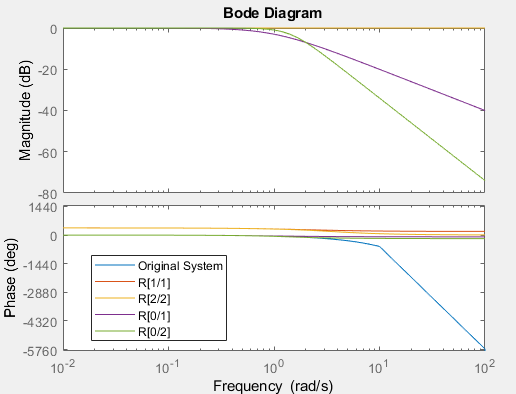
\includegraphics[width=0.7\unitlength]{images/1c}
					\caption{\label{fig:1c}The magnitude and phase responses of $e^{-s}$ and corresponding $R[0/1]$, $R[0/2]$, $R[1/1]$ and $R[2/2]$ }
				\end{figure}
				
				
		
			\item The justification hold from the previous step. The systems with non-minimum phase zeros which are R[1/1] and R[2/2] behave oscillatory behaviour around t = 0, then fit the corresponding data. The start point for non-minimum phase zeros do not fit with the original system.
		
				\begin{figure}[H]
					\center
					\setlength{\unitlength}{\textwidth} 
					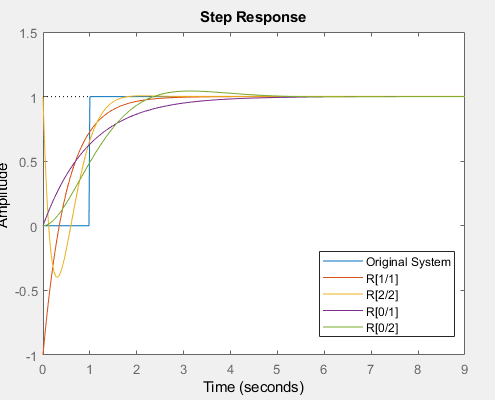
\includegraphics[width=0.7\unitlength]{images/1d}
					\caption{\label{fig:1c}The  step responses of $e^{-s}$ and corresponding $R[0/1]$, $R[0/2]$, $R[1/1]$ and $R[2/2]$ }
				\end{figure}
			
				
		
			\end{enumerate}
			
			\item  Model-Based Design Methods

	
				\begin{figure}[H]
					\center
					\setlength{\unitlength}{\textwidth} 
					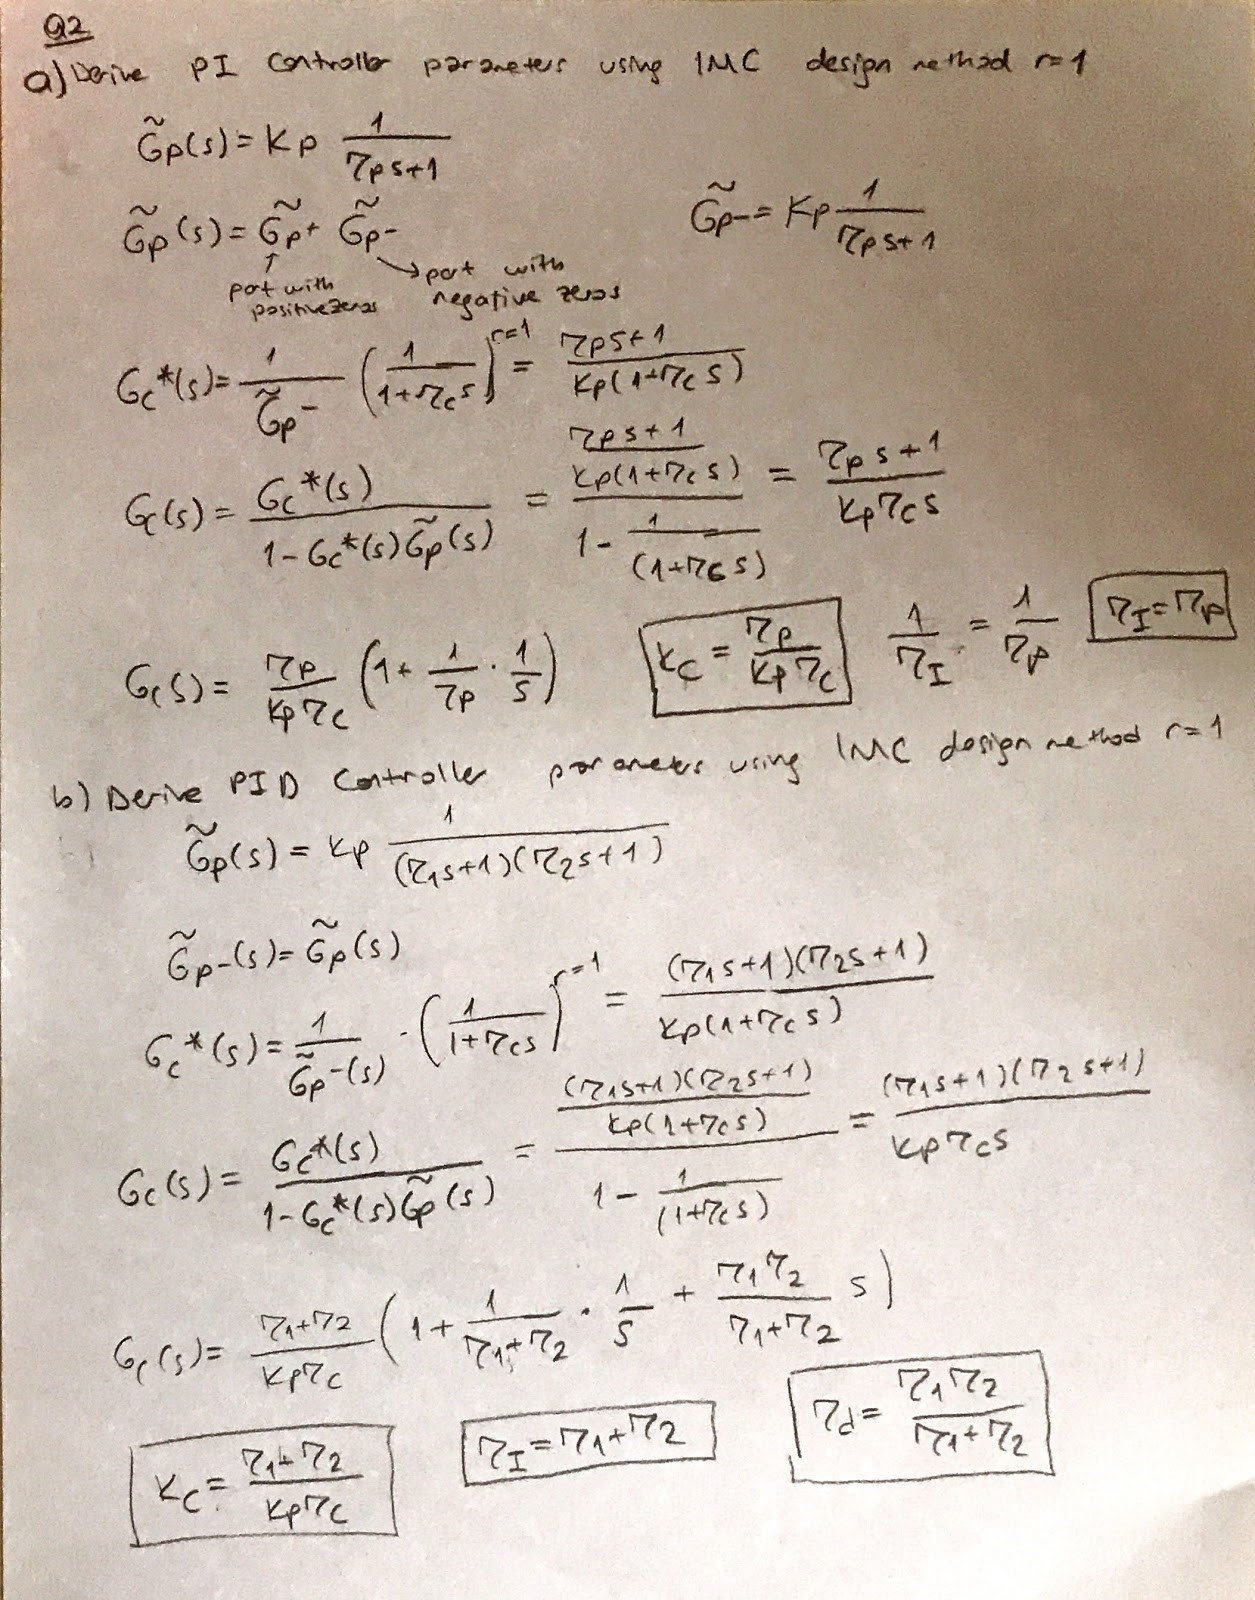
\includegraphics[width=1.0\unitlength]{images/2ab}
				\end{figure}
				\begin{figure}[H]
					\center
					\setlength{\unitlength}{\textwidth} 
					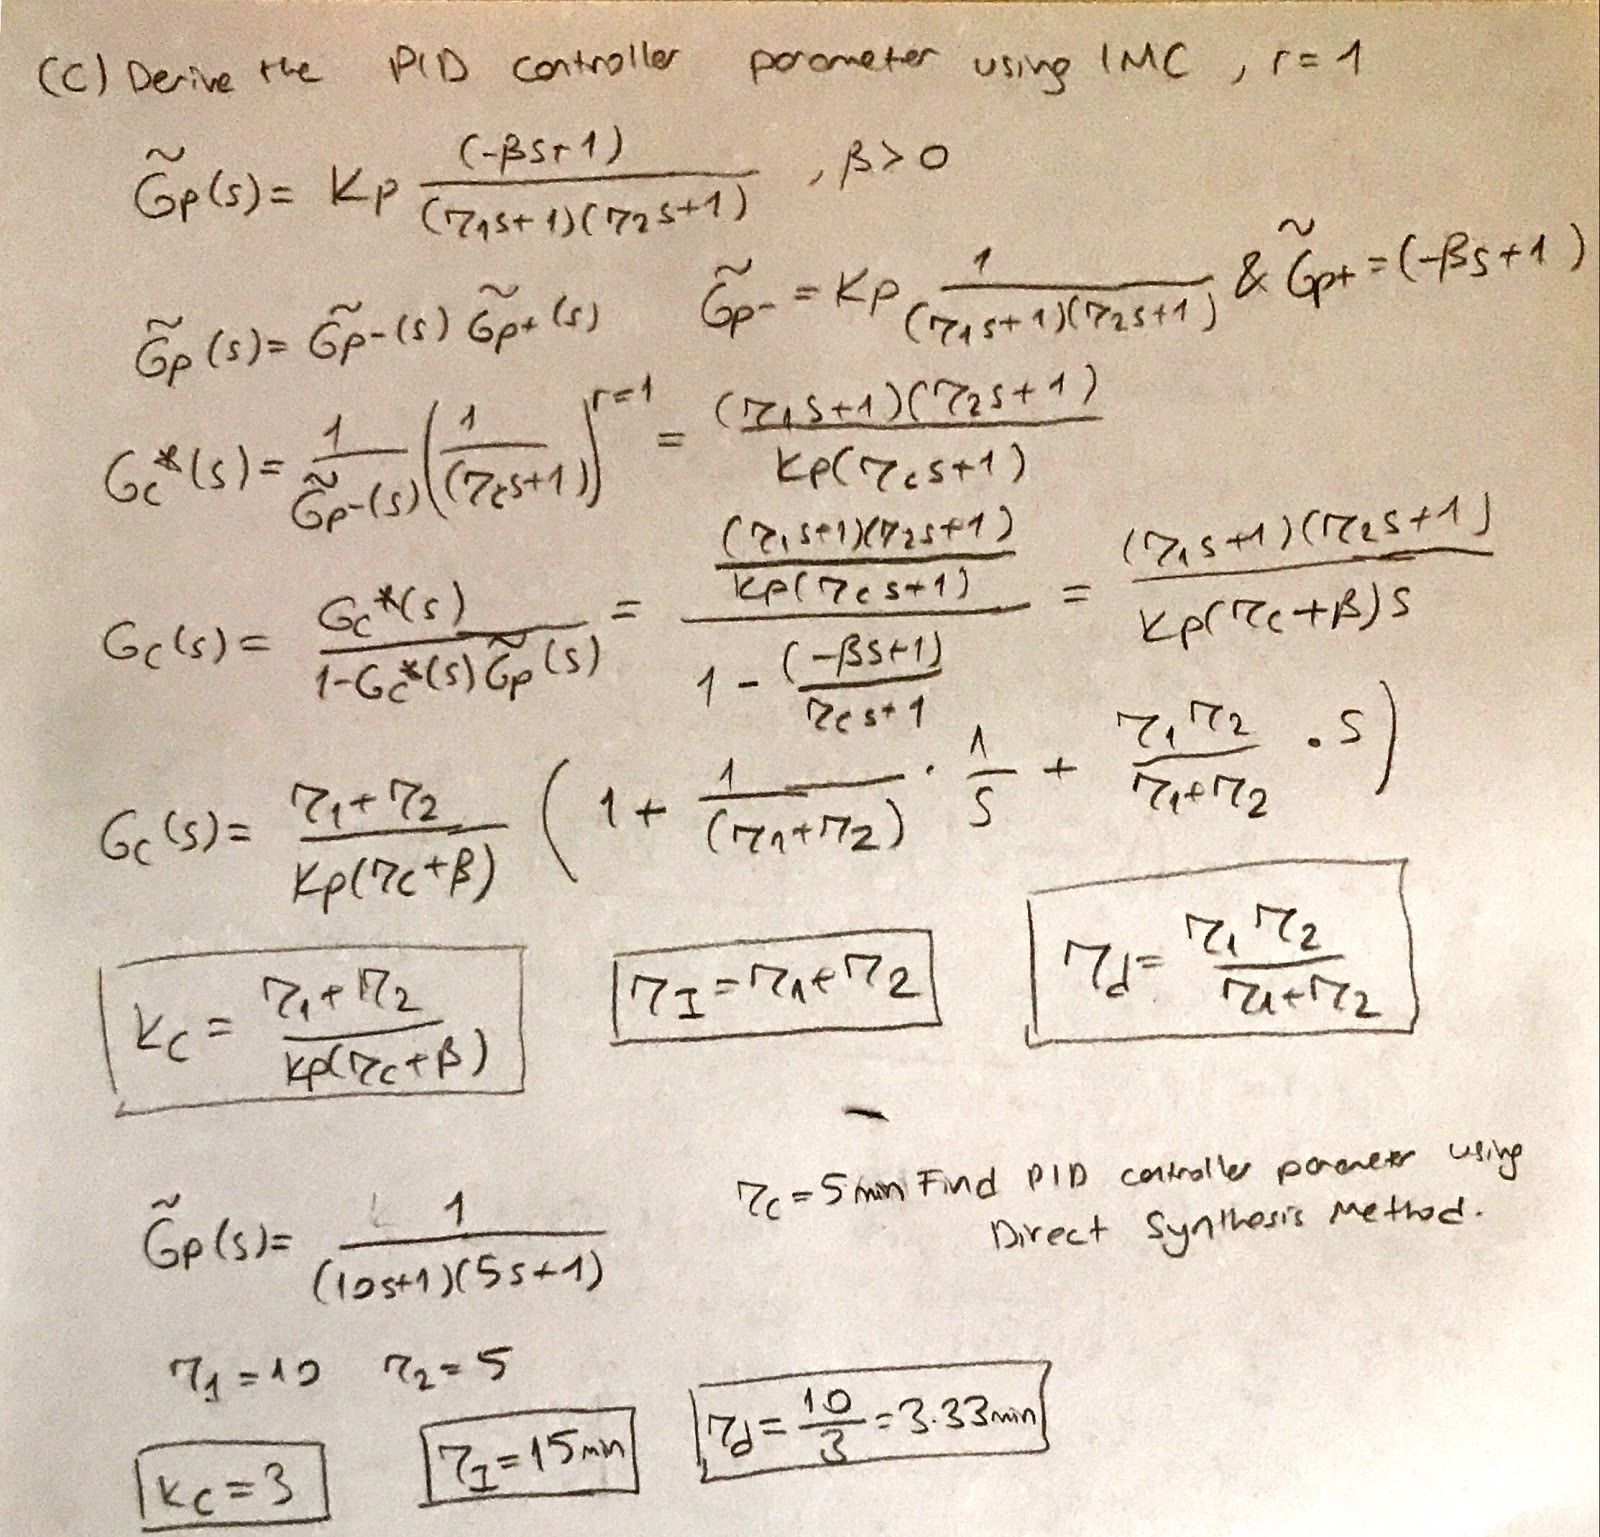
\includegraphics[width=1.0\unitlength]{images/2c}
				\end{figure}
				\begin{figure}[H]
					\center
					\setlength{\unitlength}{\textwidth} 
					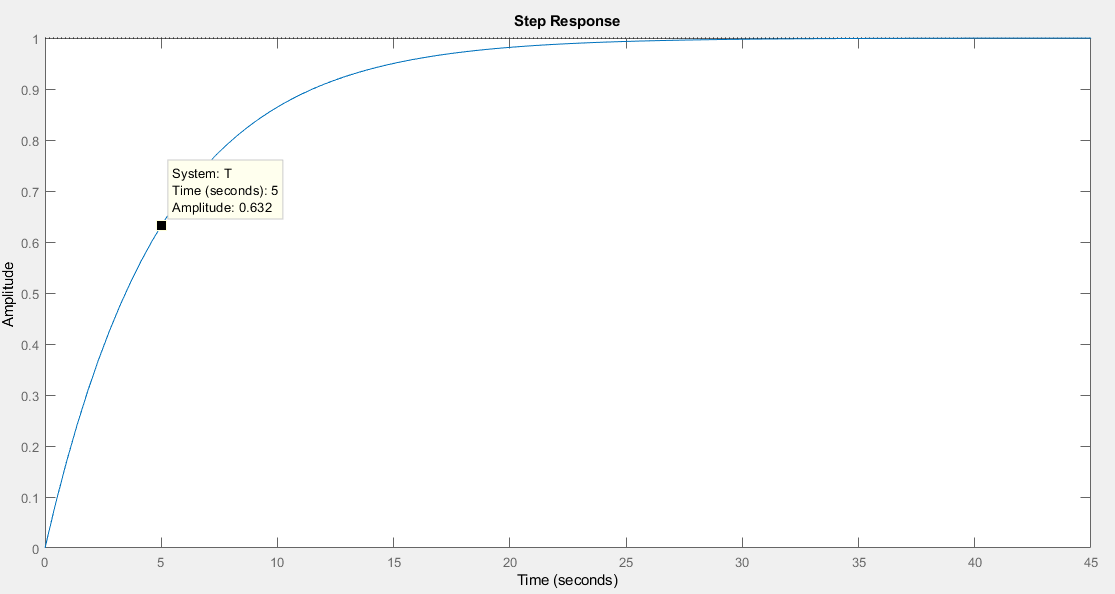
\includegraphics[width=1.0\unitlength]{images/2d}
					\caption{\label{fig:2d}The step response of  the system in Part c
The time is in minute , not in second. I write the coefficient according to minute.}
				\end{figure}
				\begin{figure}[H]
					\center
					\setlength{\unitlength}{\textwidth} 
					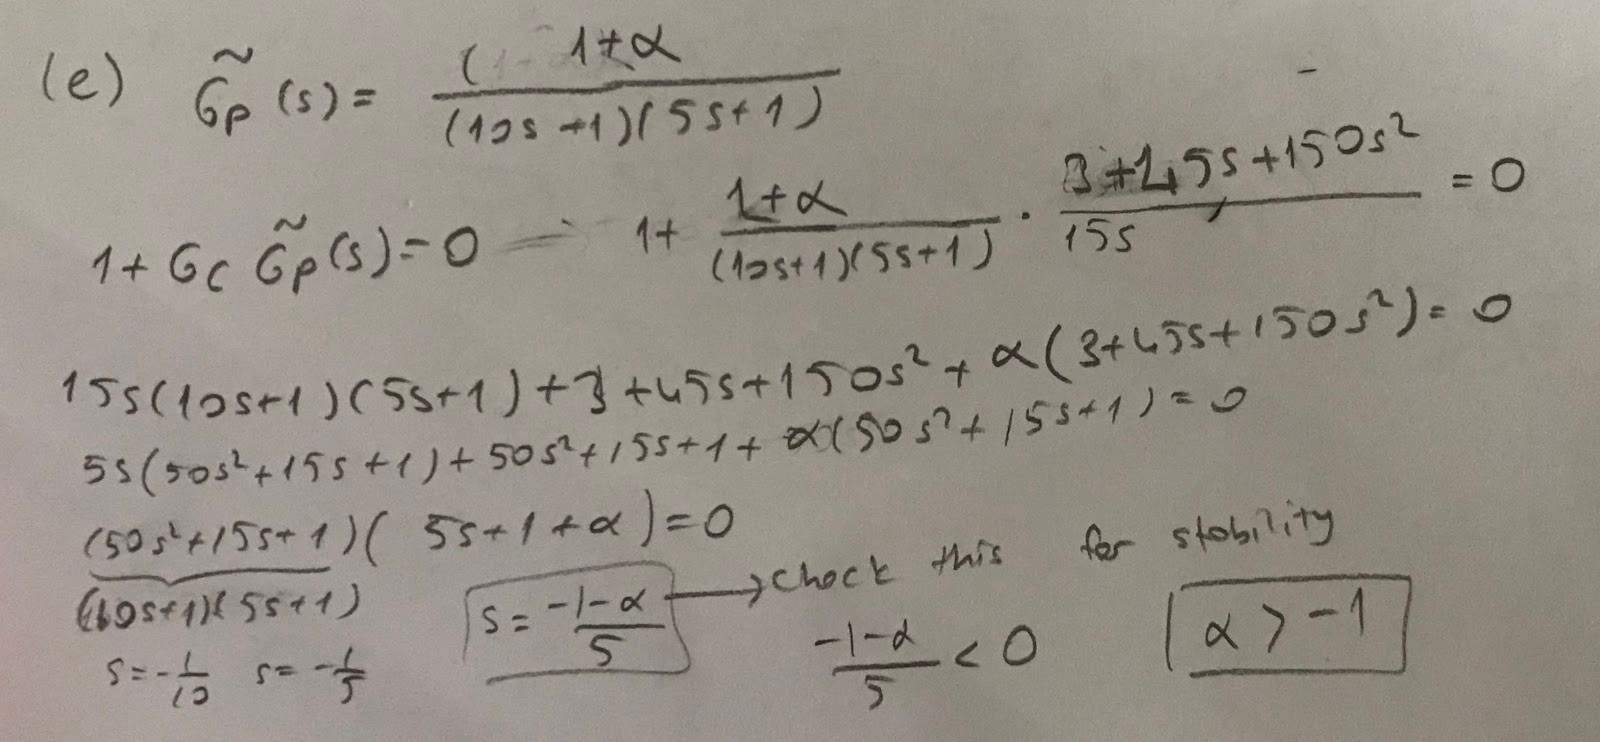
\includegraphics[width=1.0\unitlength]{images/2e}
				\end{figure}
				\begin{figure}[H]
					\center
					\setlength{\unitlength}{\textwidth} 
					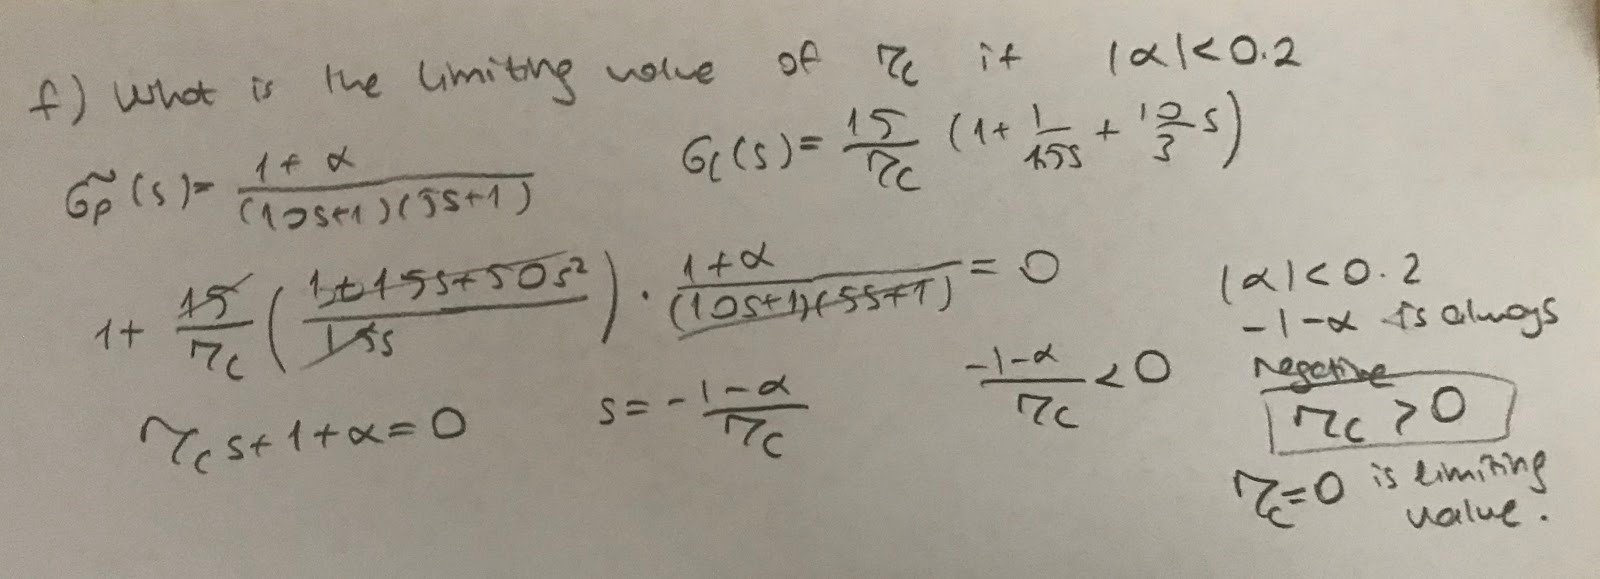
\includegraphics[width=1.0\unitlength]{images/2f}
				\end{figure}

			\item Distributed Parameter Systems
			
				\begin{figure}[H]
					\center
					\setlength{\unitlength}{\textwidth} 
					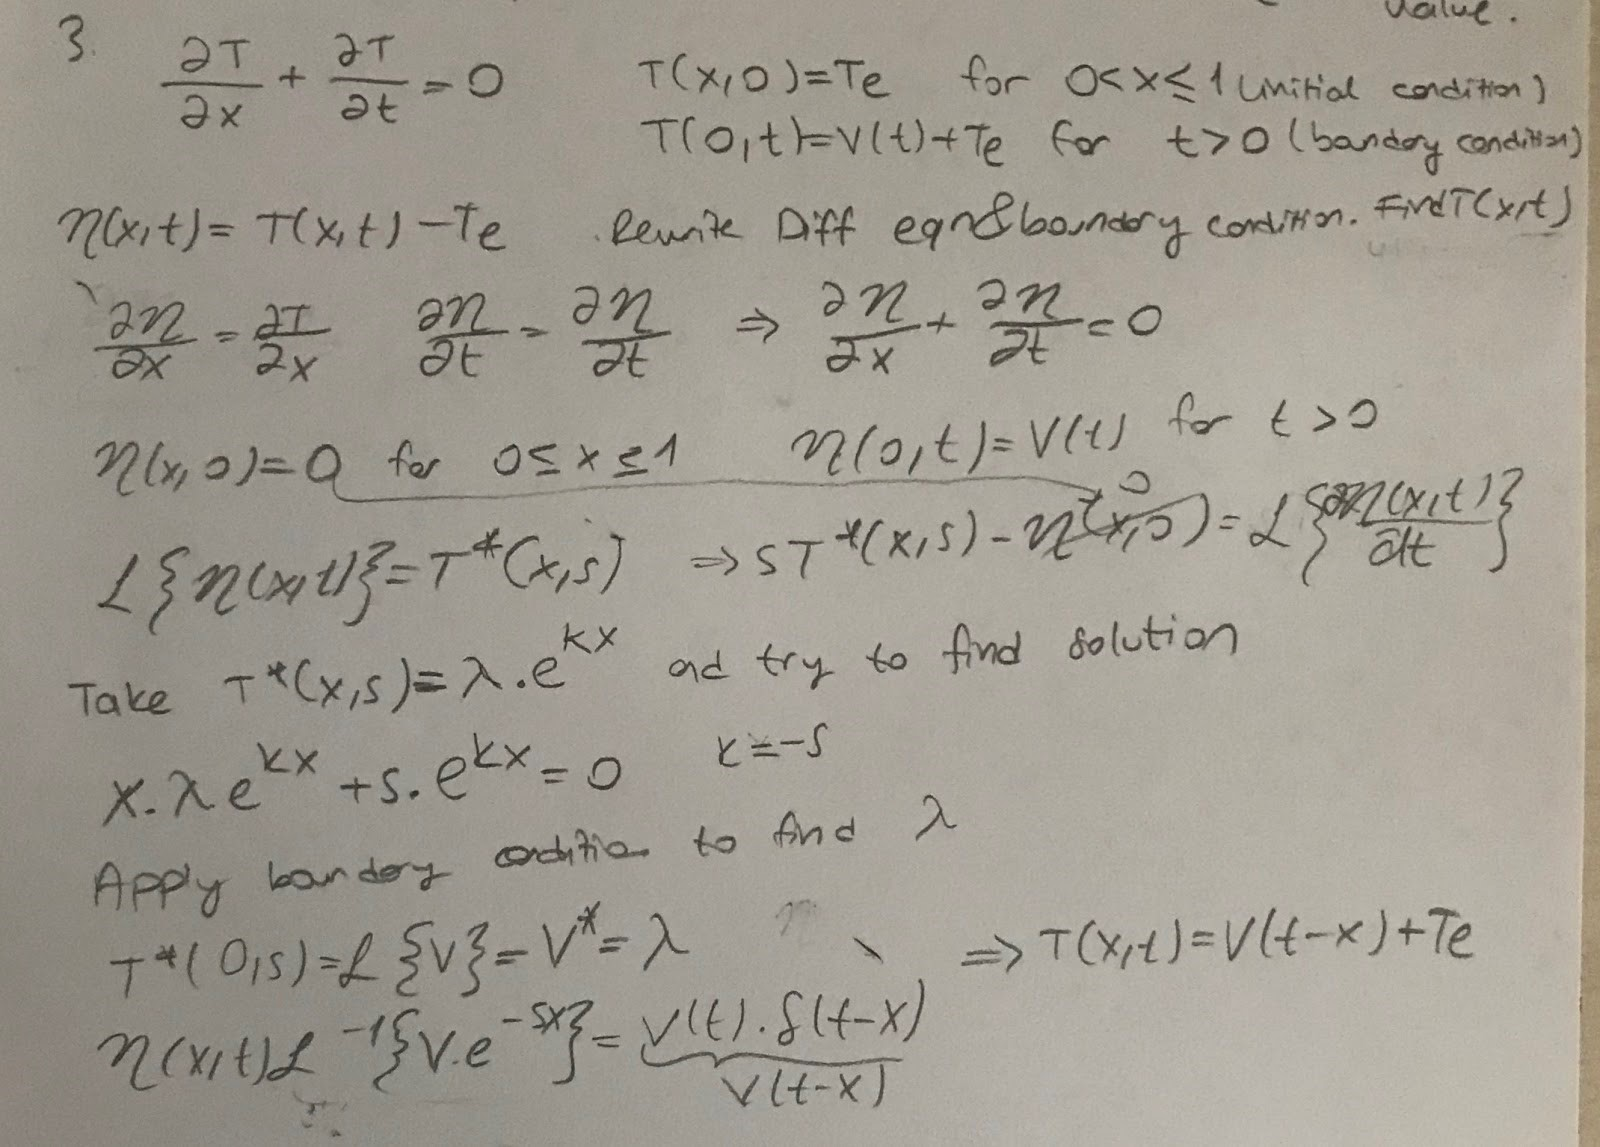
\includegraphics[width=1.0\unitlength]{images/3}
				\end{figure}
				
			\item Feedforward Control
			
				\begin{figure}[H]
					\center
					\setlength{\unitlength}{\textwidth} 
					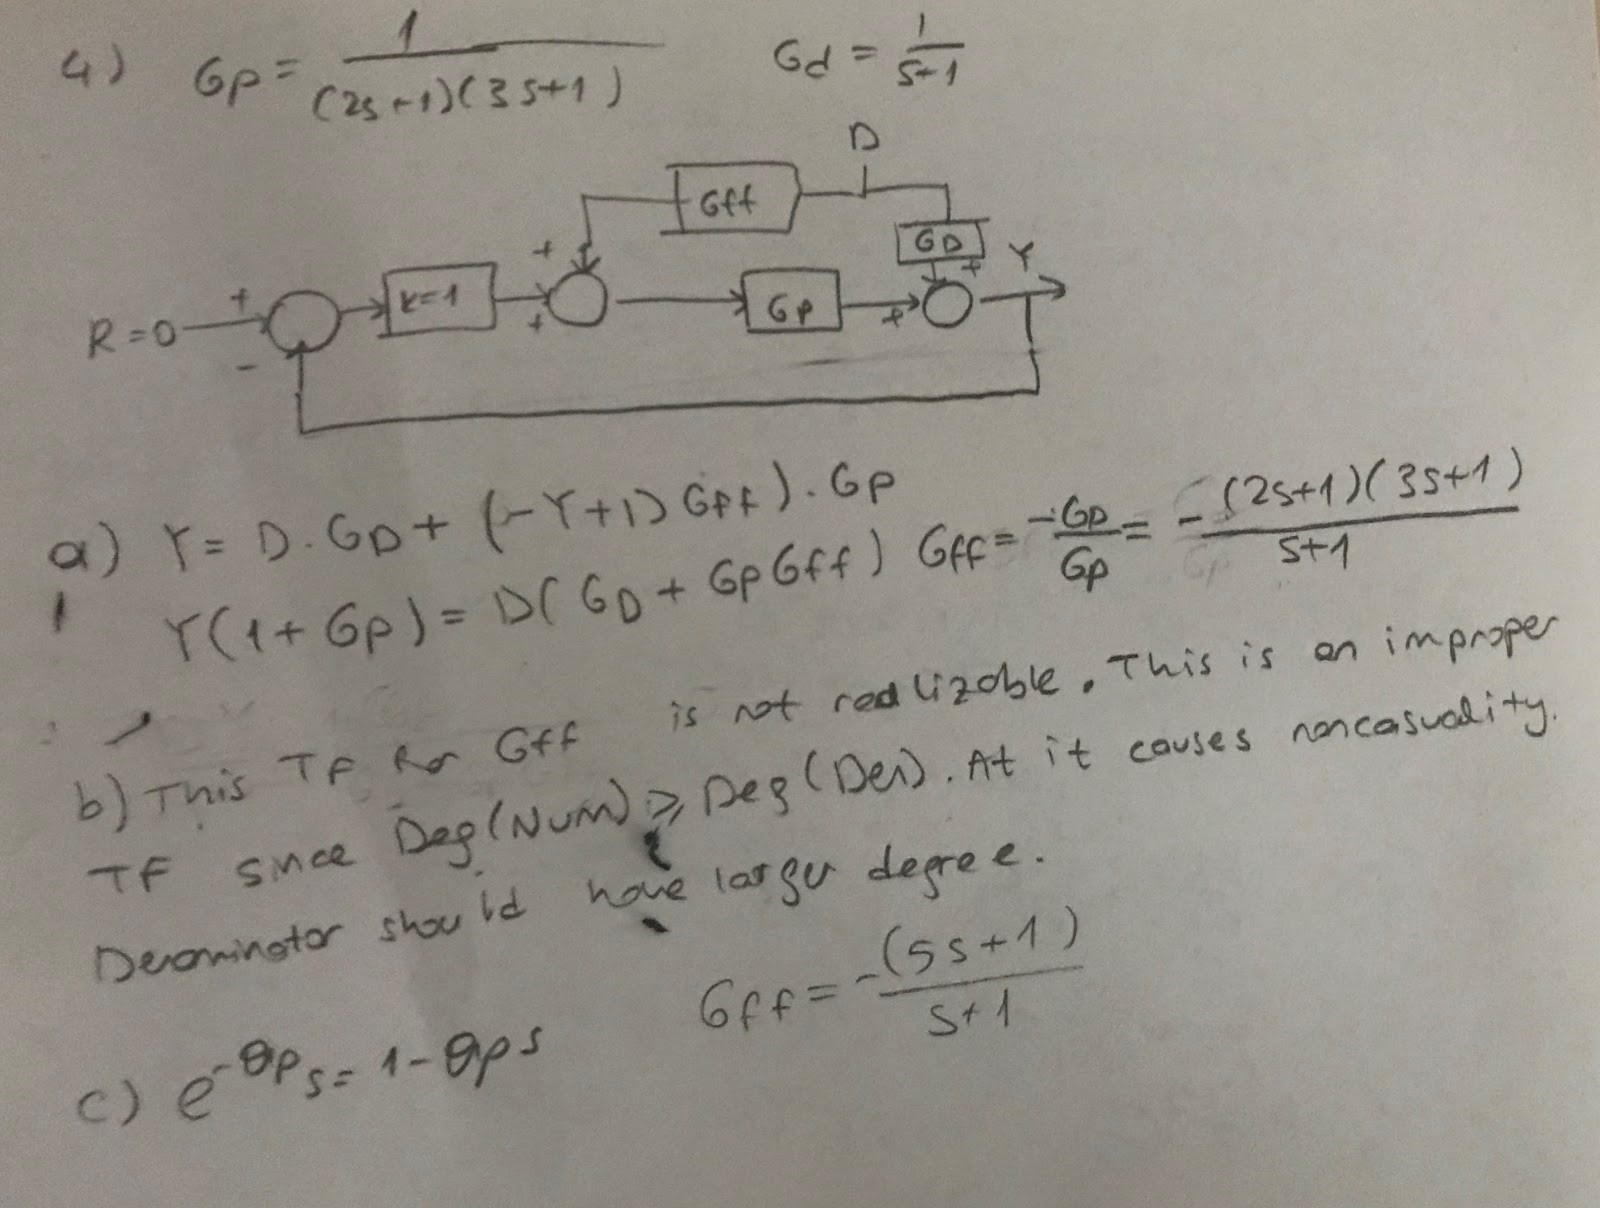
\includegraphics[width=1.0\unitlength]{images/4abc}
				\end{figure}
				
			\textbf{d)} The simulink diagram for the system can be seen at \textit{Figure~\ref{fig:simu}}. The results agrees with the expectations, as the feedforward controller added to the system, the steady state error due to step disturbance was compensated. The results can be seen at \textit{Figure~\ref{fig:ff}}.
			
				\begin{figure}[H]
					\center
					\setlength{\unitlength}{\textwidth} 
					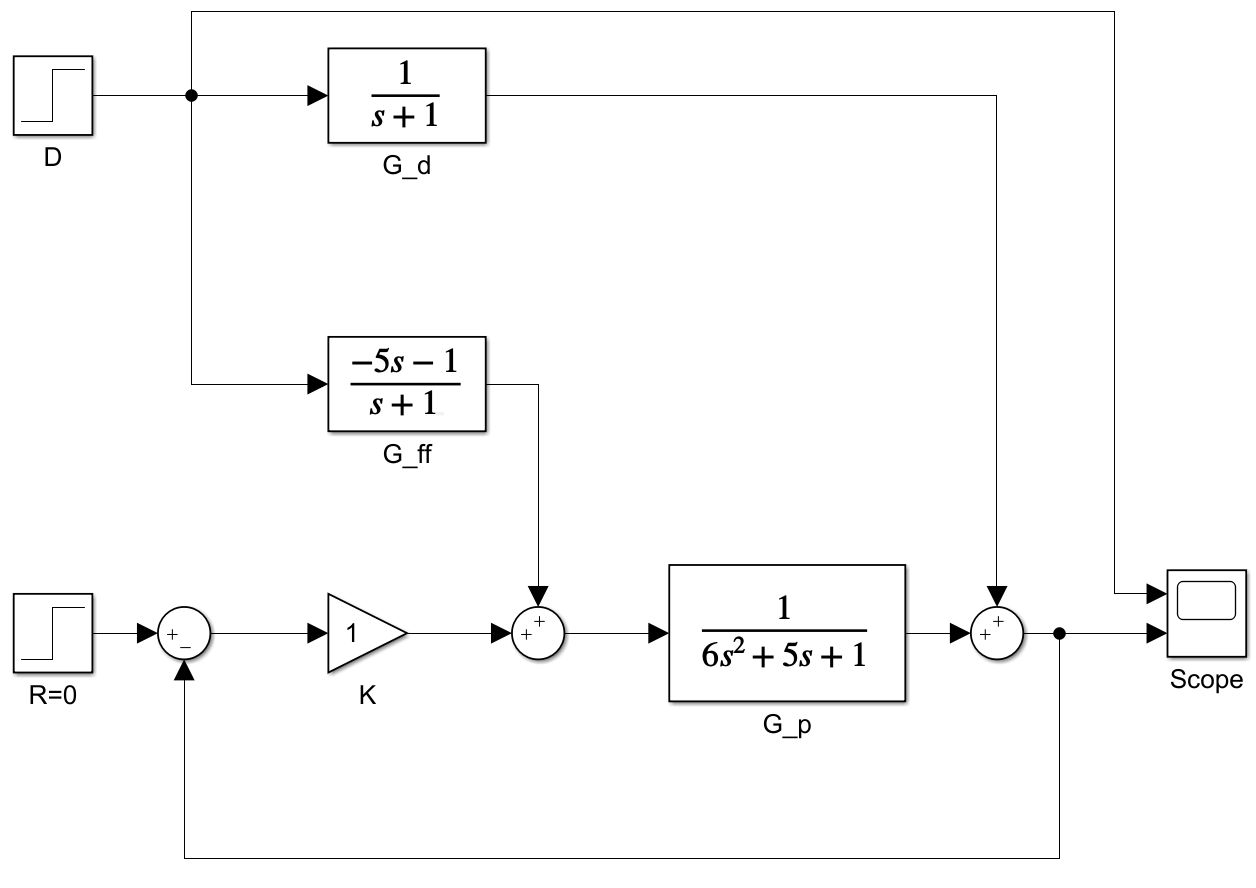
\includegraphics[width=0.6\unitlength]{images/q4}
					\caption{\label{fig:simu} Simulink Model for the System   }
				\end{figure}
				
\begin{figure}[H]
	\setlength{\unitlength}{\textwidth} 
	\centering
	\begin{subfigure}{.5\textwidth}
  		\centering
  		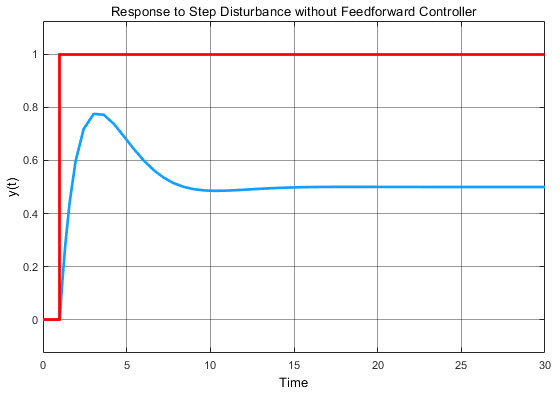
\includegraphics[width=0.48\unitlength]{images/without_ff}
  		\caption{\label{fig:withoutff}Response to Step Disturbance without Feedforward Controller }
	\end{subfigure}%
	\begin{subfigure}{.5\textwidth}
  		\centering
		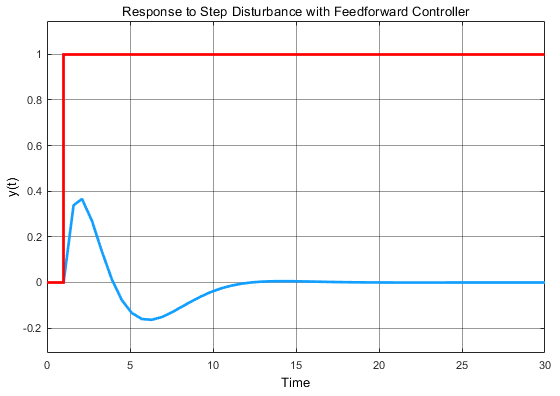
\includegraphics[width=0.48\unitlength]{images/with_ff}
  		\caption{\label{fig:withff}Response to Step Disturbance with Feedforward Controller}
	\end{subfigure}
\caption{\label{fig:ff} Response to Step Disturbance  }   
\end{figure}

	\item -
	
		\begin{enumerate}
		
			\item The open loop and closed loop transfer functions for the inner loop are
	
				$$ G_{OL,inner}=G_{c2}G_v=\frac{20}{s+1}$$
		
				$$ G_{CL,inner}=\frac{G_{c1}G_v}{1+G_{m2}G_{c2}G_v}=\frac{\frac{20}{s+1}}{1+\frac{4}{s+1}}=\frac{20}{s+5}=\frac{4}{0.2s+1}$$  
		
				as can be seen from the transfer functions also, the time constant of closed loop is five time faster than that of open loop's.
				
			\item 
			
			
			\item with given constants closed loop transfer function of the system becomes
			
				$$ G_{CL}=\cfrac{G_{c2}(\cfrac{4}{0.2s+1})G_p}{1+G_{c1}\cfrac{4}{0.2s+1}G_pG_{m1}}$$
				$$ G_{CL}= \cfrac{G_{c2}(\cfrac{20}{s+5})(\cfrac{4}{(4s+1)(2s+1)})}{1+G_{c1}(\cfrac{20}{s+5})(\cfrac{4}{(4s+1)(2s+1)})0.05}$$
				
				Then characteristic equation becomes \textit{(for D=0);}
				
				$$ q(s)=1+G_{c1}\left(\cfrac{4}{(s+5)(4s+1)(2s+1)}\right)=0$$
				
				$$ (s+5)(4s+1)(2s+1) +4 G_{c1}=0 $$
				
				$$ 8s^3 + 46s^2 + 31^s + 5 + 4 G_{c1} =0$$
				
				From Routh-Hurwitz stbility crietarian, critical gain $G_{c1}$ can be found as
				
				$$ G_{c1,max}= 43.31 $$
				
				$$\boxed{ K_c \approx \frac{G_{c1,max}}{2}=21.66 }$$
				
				\item with given numbers, the CLTF becomes
				
				$$ G_{CL}=\cfrac{4(\cfrac{5}{s+1})\cfrac{4}{(4s+1)(2s+1)}}{1+\cfrac{5}{s+1}\cfrac{4}{(4s+1)(2s+1)}0.05}$$
				
				Then characteristic equation becomes \textit{(for D=0);}

				$$ 	q(s)= 1+G_{c1}\cfrac{1}{(s+1)(4s+1)(2s+1)} $$
				
				$$ (s+1)(4s+1)(2s+1)+G_{c1}=0$$
				
				$$ 8s^3 + 14s^2 + 7^s + 1 +G_{c1}=0 $$
				
				Again from Routh-Hurwitz
				
				$$ G_{c1,max}= 11.25  $$
				
				$$\boxed{ K_c \approx \frac{G_{c1,max}}{2}=5.625 }$$
				
				\item 
				
					$$ E_1G_{c1}-Y_2G_{m2}=E_2$$
					
					$$ E_2G_{c2}G_v+D=Y_2$$
					
					Assuming $R=0$
					
					$$ E_1=-G_{m1}G_pY_2$$	
					
					$$ -G_{c1}G_{m1}G_pY_2-Y_2G_{m2}=E_2$$
					
					$$ Y_2=\frac{-1}{G_{c1}G_{m1}G_p+G_{m2}}E_2$$
					
					$$ D=-E_2G_{c2}G_v+\frac{-1}{G_{c1}G_{m1}G_p+G_{m2}}E_2$$
					
					$$ E_2(s)=\cfrac{-D(s)}{E_2G_{c2}G_v+\cfrac{1}{G_{c1}G_{m1}G_p+G_{m2}}}$$
				
					with $D(s)=\frac{1}{s}$
					
					$$ e_{2,ss}=\lim_{s \to 0} sE_2(s)(\cfrac{-}{E_2G_{c2}G_v+\cfrac{1}{G_{c1}G_{m1}G_p+G_{m2}}})$$
					
					with controller ($G_{c2}=4$ $G_{m2}=0.2$)
					
					$$ e_{2,ss} \approx -0.0022 $$

					without controller ($G_{c2}=1$ $G_{m2}=0$)
					
					$$ e_{2,ss} \approx -0.0302 $$
					
				The simulink diagram for the system can be seen at \textit{Figure~\ref{fig:simu5}}. The results agrees with the expectations, as the inner controller added to the system, the steady state error due to step disturbance was almost compensated. The results can be seen at \textit{Figure~\ref{fig:in}}.
			
				\begin{figure}[H]
					\center
					\setlength{\unitlength}{\textwidth} 
					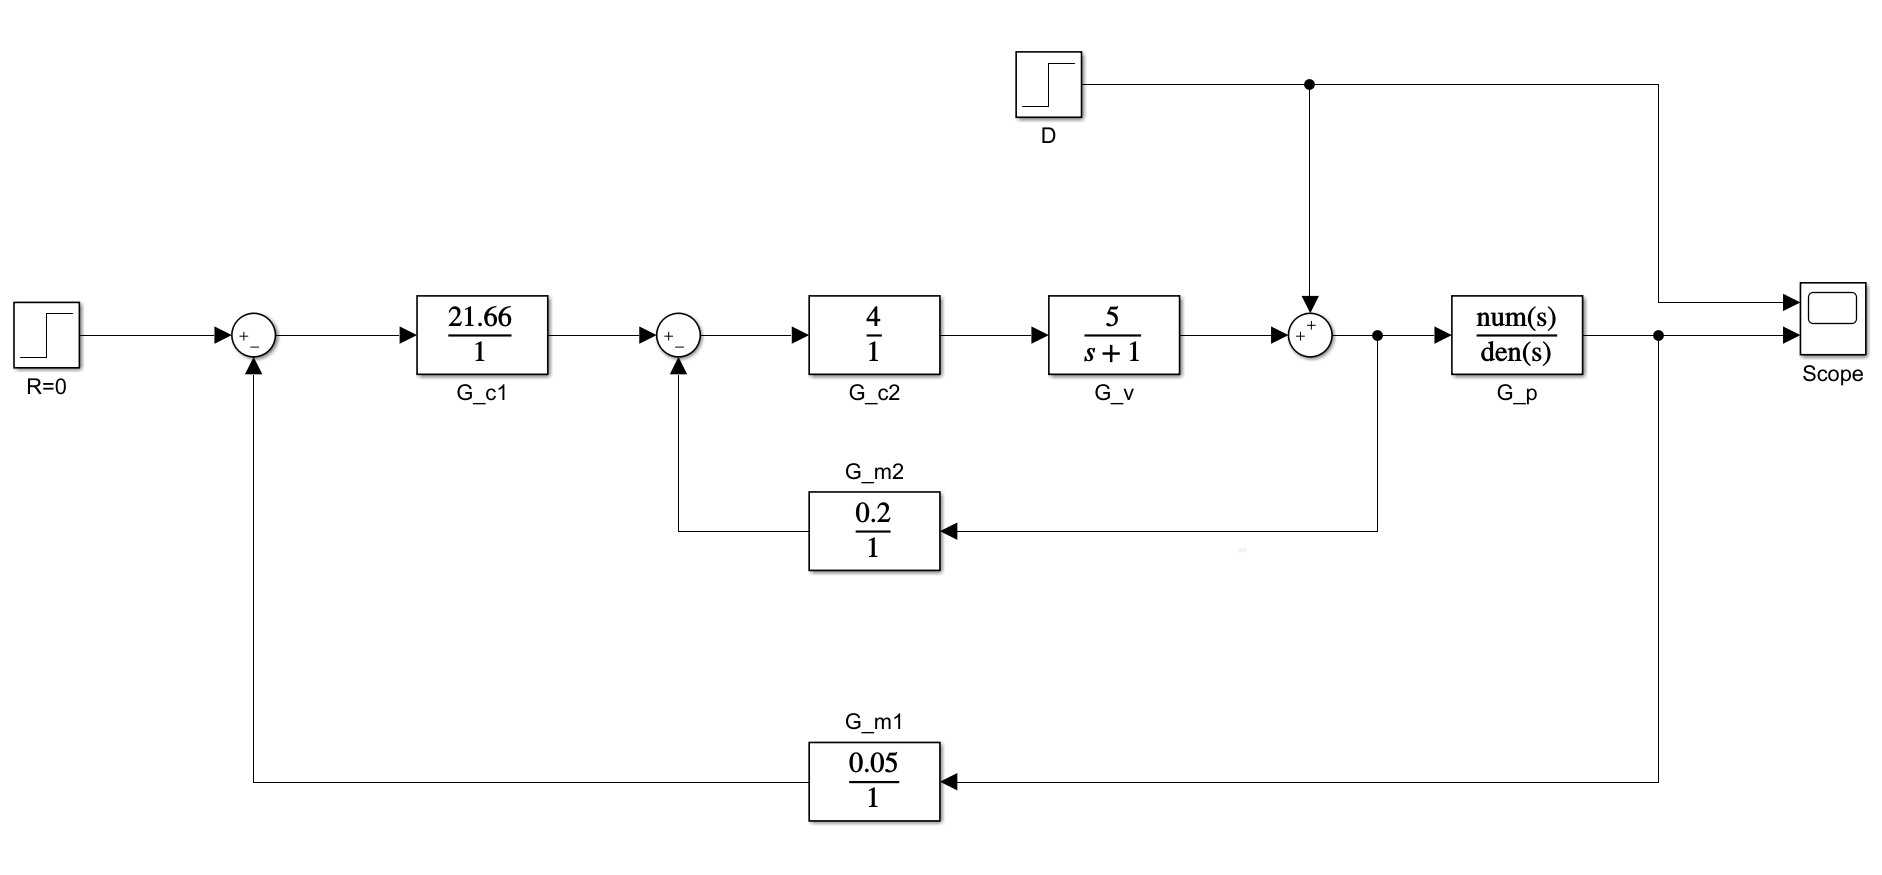
\includegraphics[width=0.6\unitlength]{images/q5}
					\caption{\label{fig:simu5} Simulink Model for the System   }
				\end{figure}
				
\begin{figure}[H]
	\setlength{\unitlength}{\textwidth} 
	\centering
	\begin{subfigure}{.5\textwidth}
  		\centering
  		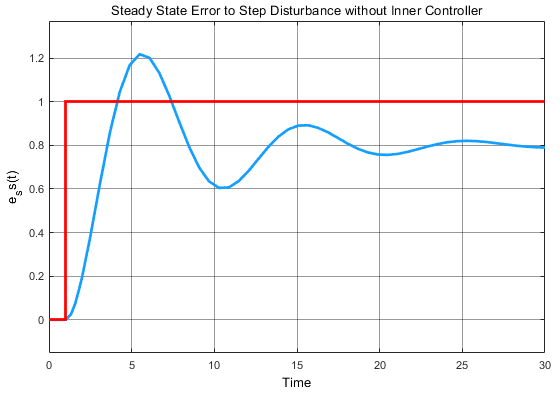
\includegraphics[width=0.48\unitlength]{images/without_in}
  		\caption{\label{fig:withoutff}Response to Step Disturbance without Inner Controller }
	\end{subfigure}%
	\begin{subfigure}{.5\textwidth}
  		\centering
		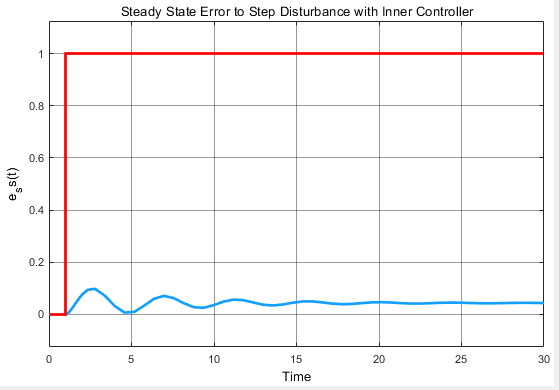
\includegraphics[width=0.48\unitlength]{images/with_in}
  		\caption{\label{fig:withff}Response to Step Disturbance with Inner Controller}
	\end{subfigure}
\caption{\label{fig:in} Response to Step Disturbance  }  
\end{figure}

	\item System become more stable and less oscillatory with the addition of Cascade Controller. The error rejectşon ratio increased significantly.
					
				
 
			
			
			
			
		
		\end{enumerate}
		
	\end{enumerate}

%\newpage		
%\begin{appendices}
%\section{Source Code for Matlab Part of Question 2 }\label{appendix}
	%%	\lstinputlisting[language=Matlab,firstline=33, lastline=34]{q13.m} \-\\[1cm]		
%\lstinputlisting[language=Matlab]{..//Q2.m} 
%\end{appendices}
	
	
	
\end{document}

%----samples------
%\begin{itemize}
%\item Item
%\item Item
%\end{itemize}

%\begin{figure}[H]
%\center
%\setlength{\unitlength}{\textwidth} 
%\includegraphics[width=0.7\unitlength]{images/logo1}
%\caption{\label{fig:logo}Logo }
%\end{figure}

%\begin{figure}[H]
%	\setlength{\unitlength}{\textwidth} 
%	\centering
%	\begin{subfigure}{.5\textwidth}
%  		\centering
%  		\includegraphics[width=0.48\unitlength]{images/logo1}
%  		\caption{\label{fig:logo1}Logo1 }
%	\end{subfigure}%
%	\begin{subfigure}{.5\textwidth}
%  		\centering
%		\includegraphics[width=0.48\unitlength]{images/logo2}
%  		\caption{\label{fig:logo2}Logo2}
%	\end{subfigure}
%\caption{\label{fig:calisandegree} Small Logos   }
%\end{figure}
	
%\begin{table}[H]
%  \centering
% 
%    \begin{tabular}{c|c|c}
%       $$A$$ & $$B$$ & $$C$$ \\ \hline
%       1 & 2 & 3  \\ \hline
%       2 & 3 & 4  \\ \hline
%       3 & 4 & 5  \\ \hline
%       4 & 5 & 6  
%      
%  \end{tabular}
%  \caption{table}
%  \label{tab:table}
%\end{table}
	
%\begin{table}[H]
%  \centering
% 
%    \begin{tabular}{c|c|c}
%       \backslashbox{$A$}{$a$} & $$\specialcell{ Average deviation \\ after subtracting out the  \\ frequency error }$$ & $$C$$ \\ \hline
%       \multirow{2}{*}{1} & 2 & 3  \\ \cline{2-3}
%        & 3 & 4  \\ \hline
%       3 & \multicolumn{2}{c}{4}  \\ \hline
%       4 & 5 & 6  
%      
%  \end{tabular}
%  \caption{table}
%  \label{tab:table}
%\end{table}
%-----end of samples-----